\documentclass[11pt,a4paper]{article}

\usepackage[T1]{fontenc}
\usepackage[utf8]{inputenc}
\usepackage[frenchb]{babel}

\usepackage{fancyhdr} % headers
\usepackage[usenames,dvipsnames]{color} % colors
\usepackage{graphicx} % images
\usepackage{listings} % source code
\usepackage{titling} % meta-infos
\usepackage{courier} % courier font
\usepackage{fullpage} % full page layout
\usepackage{titlesec} % title customization
\usepackage{parskip} % paragraphs spacing
\usepackage{amsmath}
\usepackage{tikz}
\usepackage{siunitx}
%\usepackage{showframe} % layout debug

\usepackage{float}
\restylefloat{figure}

\topmargin -10mm
\headsep 5mm
\headheight 10mm

\linespread{1.1}
\renewcommand{\arraystretch}{1.3}

\setlength\parindent{0pt}
\setlength{\unitlength}{1cm}
\setlength{\droptitle}{-1.6cm}

\pagestyle{fancy}
\fancyhf{}
\cfoot{\thepage}

\def \doccourse { TIB1-B }
\def \doctitle {Rapport : Routage dynamique}
\author{Bastien Clément \and Christophe Peretti}

\renewcommand{\thesection}{Objectif \arabic{section} :}
\renewcommand{\thesubsection}{\arabic{section}.\arabic{subsection}}

\rhead{\theauthor \\ \today}
\lhead{\doccourse \\ \doctitle }
\title{{\normalsize \doccourse} \\ \doctitle }

\begin{document}

\maketitle
\vspace{1em}

\section{Analyse de la mise à jour des routes}

L'objectif de cette partie est de comprendre le mécanisme de mise à jour des routes. Il est atteint si nous savons expliquer le fonctionnement de la mise à jour des tables de routage lors du changement du statut d’un lien.

\subsection{Simulation de la panne du lien}

\subsubsection*{Combien de temps la transmission est-elle interrompue ?}

Le lien est déactivé aux alentours de \texttt{00:20:00}. Le routeur se rend compte que le lien est defectueux, met à jour sa table de routage puis averti ses voisins à \texttt{00:23:14}. La transmission entre l'ordinateur local et le serveur de Google est donc impossible pendant plus ou moins 3 minutes.

\subsubsection*{Diagramme chronologique des événements}

\begin{center}
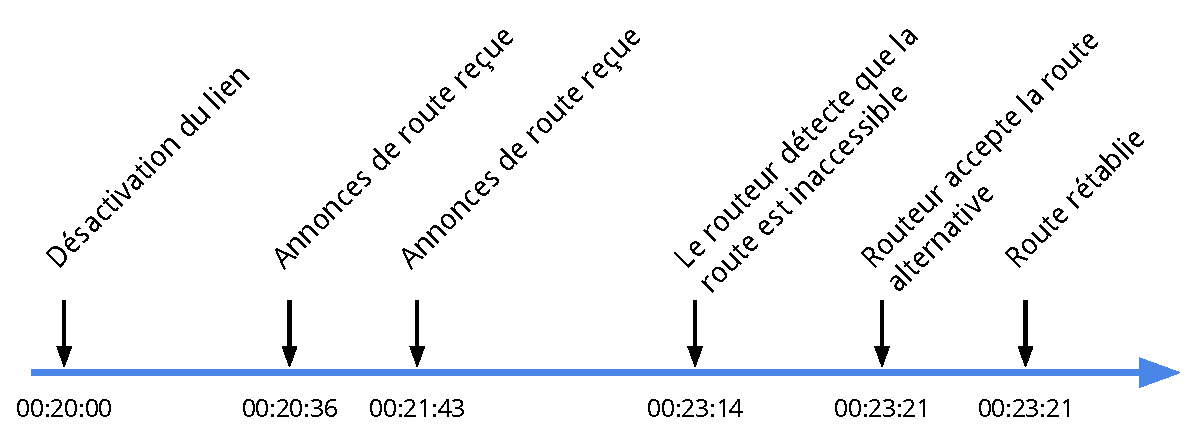
\includegraphics[width=13cm]{img_down}
\end{center}

On observe ici que le routeur requiert un temps relativement long, 3 minutes, pour considérer un lien comme défaillant et mettre à jour sa table de routage.

Ce délai est probablement conçu pour éviter des mises à jours trop fréquentes des tables de routages en cas de coupure brève du lien entre deux routeurs.

Après trois minutes, le lien est considéré défaillant et la table de routage est mise à jour en coopération avec les routeurs voisins pour rétablir la communication sur une route alternative.

\subsection{Réactivation du lien}

\subsubsection*{Est-ce que la transmission est interrompue ?}

Dans cette deuxième parties du laboratoire, la transmission n'est jamais interrompue.

À l'inverse de la première partie où les routeurs étaient temporairement configurés pour utiliser une route défaillante, la route qu'ils utilisent est parfaitement fonctionnelle même si non-optimale. La retour sur le lien réactivé se fait de façon transparente pour le trafic.

\subsubsection*{Diagramme chronologique des événements}

\begin{center}
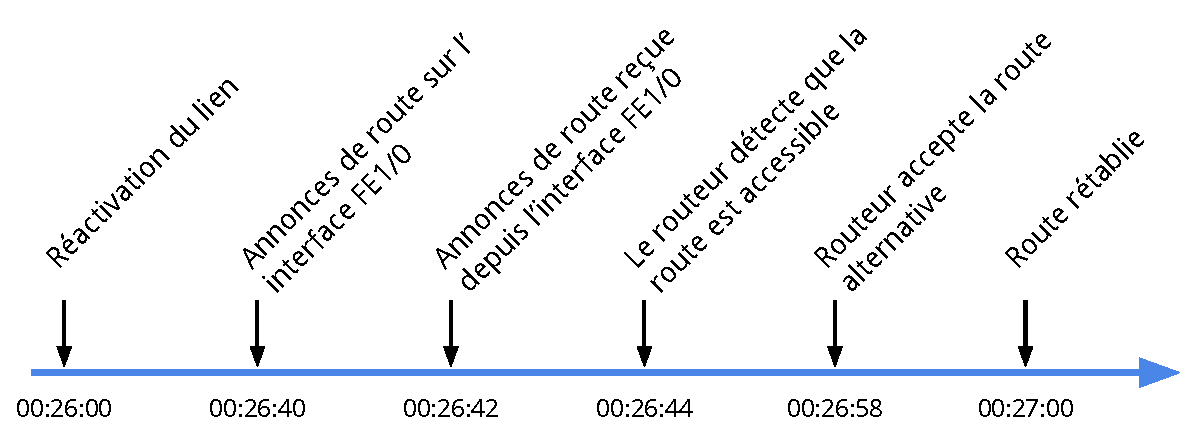
\includegraphics[width=13cm]{img_up}
\end{center}

La détection de réactivation du lien est bien plus rapide. En effet, dès le premier échange résussi sur ce lien, ce dernier est considéré comme à nouveau fonctionnel et les tables de routages sont mises à jour. Par la suite, le trafic entre notre machine local et le serveur de Google empruntera à nouveau la route optimale.

Comme toutes les routes de sont pas mises à jour simultanément, il est possible que, pendant un moment, les deux directions n'emprunte par la même route. C'est à dire que la trafic de notre machine au serveur emprunte la route optimale, alors que le trafic en sens inverse utilise encore temporairement la route non-optimale. Ceci n'impacte pas la communication entre les deux noeuds puisque les paquets parviennent, dans les deux cas, aux destinataires.

\section{Auto-évaluation}

Nous considérons avoir atteint les objectifs de ce laboratoire.

\end{document}